
\chapter{Methodology}

\section{Dataset Pre-Processing}
The dataset used in this study is the transactional sales data from a chain of Brazilian gas-station stores \cite{data_source}.
Each row in the dataset represents the purchase of a specific product as part of a transaction - and as such, each row corresponds to the following columns:
\begin{itemize}
\item Company Code
\item Order Number
\item Employee
\item Product
\item Product Category
\item Client
\item Sale Date Time
\item Product Cost
\item Discount Amount
\end{itemize}
All personal and corporate names were exchanged for fictitious names by the author of the dataset in order to preserve the anonymity of those whose who could have otherwise been identified through the dataset. Before employing the dataset, sanitary procedures were carried out to ensure that the dataset was error-free and in a format suitable for graph generation. The steps have been detailed below.

\begin{enumerate}
\item \textbf{Transaction Identifier}\\
The \textit{Order Number} field showed discrepancies, where a given order number could reference distinct transactions in different stores and cities, and at different dates and times. 
This could be due to the stores maintaining their own order numbers, and also because the order numbers may reset after a predetermined limit.
A unique transaction identifier - named \texttt{basket\_id} - was created by concatenating the order number and the date, thereby mitigating the occurrence of a identifier that references multiple transactions.

\item \textbf{Binary Purchase Vector transformation}\\
The dataset was then transformed such that each transaction was represented by a binary purchase vector - as described in Section \ref{sec:binary_purchase_vectors} - wherein each column represents a product category. The product categories were chosen for the graph representation over the products themselves as it would give a more generalized view on the associations between them, and the categories themselves were deemed specific enough that they would not be parent to children of significant variance.

\end{enumerate} 
\section{MST Generation}
\begin{figure}[H]
\centering
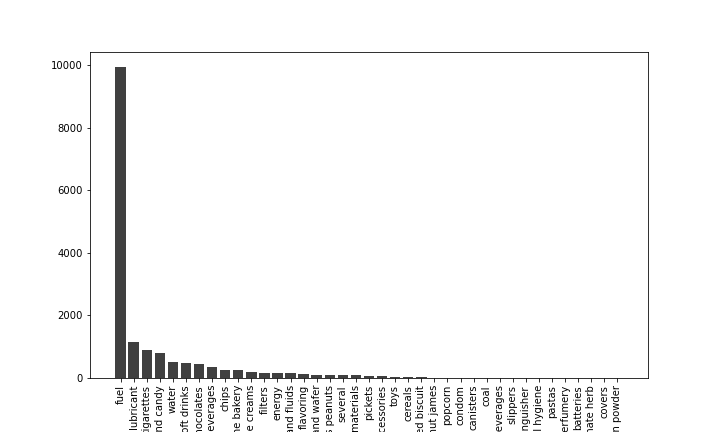
\includegraphics[scale=0.5]{category_dist}
\caption{Category Distribution}
\label{fig:cat_dist}
\end{figure}
The metrics used to assess the association rules - support, lift and confidence - are based on the proportional presence of a given itemset in the transactions. Since our dataset is from a gas-station store chain, fuel products dominate the transactional presence by a significant factor. Figure \ref{fig:cat_dist} highlights the disparity between the presence of \textit{fuel} products and the others, with \textit{fuel} being present in $99.28\%$ of all transactions. To avoid the association rules being dominated by the \textit{fuel} category - which should inherently understood to be a key product for gas stations - the fuel category was purged from the dataset.

Using the Pearson's Correlation Coefficient \cite{pearson} (Equation \ref{eq:pearson}), a correlation matrix was derived from the binary purchase vector dataset. In this instance - because the correlation is of binary variables - the Pearson's Correlation Coefficient is equivalent to the Phi Coefficient ($\phi$) \cite{phi}. The resulting correlation matrix is also diagonally symmetrical (i.e. $\phi_{ij} = \phi_{ji}$), and therefore the illustration of the correlation matrix in Figure \ref{fig:correlation} displays only those values that are below the diagonal.
\begin{equation}
\label{eq:pearson}
r = \frac{ n(\sum xy) - (\sum x) (\sum y)} { \sqrt{ [n\sum x^2 - (\sum x)^2] [n \sum y^2 - (\sum y)^2] } }
\end{equation}




\begin{figure}[H]
\centering
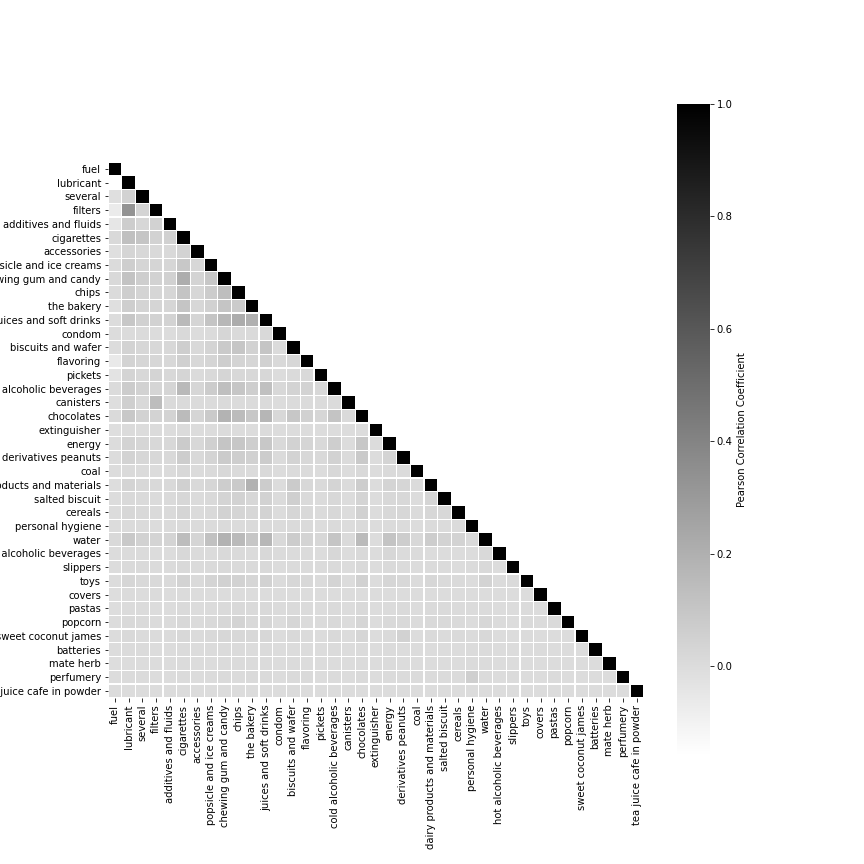
\includegraphics[scale=0.4]{correlation}
\caption{Correlation Matrix from Binary Purchase Vectors}
\label{fig:correlation}
\end{figure}

A minimum spanning tree is a graph composed of the \textit{shortest} path connecting all vertices, and therefore the values in the correlation matrix would need to be transformed via a function such that the higher the correlation value, the lower the output value. This would allow the MST to capture the strongest associations between the product categories. As used by \textbf{M. A. Valle et al.} in \cite{mst_paper}, the distance function (Equation \ref{eq:distance_function}  was used to make this transformation - where $\phi_{ij}$ refers to the correlation value for two given product categories $i$ and $j$ in Figure \ref{fig:correlation}). However, whereas \textbf{M. A. Valle et al.} left their $\phi_{ij}$ unaltered, we have converted it to an absolute value (i.e. $|\phi_{ij}|$). The reason behind this is to capture the strongest relationships between product categories, positive and negative alike. By leaving the value unaltered, the MST would not capture strong negative associations as they would have the highest weights after the distance function was applied. Figure \ref{fig:distance_function} illustrates the effect of this function, where the stronger the correlation, the lower the distance function's output. The figure also demonstrates that because the Pearson's Correlation Coefficient is bound to the interval $[-1,1]$, the distance function's output is therefore bound to the interval $[0,\sqrt{2}]$. 
\begin{equation}
\label{eq:distance_function}
d_{ij} = \sqrt{2(1-|\phi_{ij}|)}
\end{equation}

\begin{figure}[H]
\centering
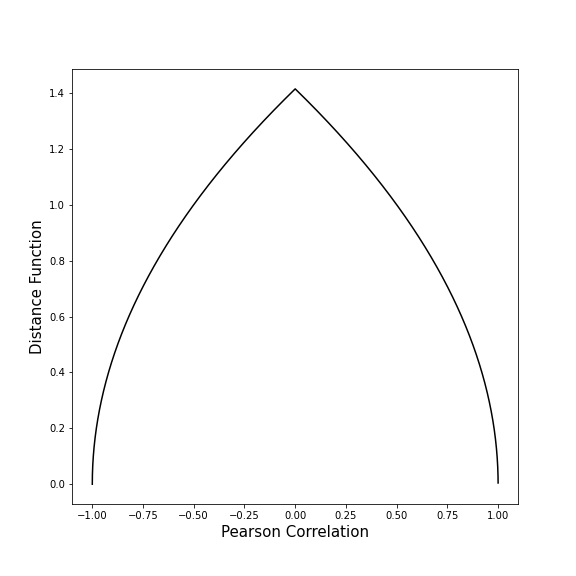
\includegraphics[scale=0.4]{distance_function}
\label{fig:distance_function}
\caption{The effect of the distance function $\sqrt{2(1-|x|)}$}
\end{figure}

\begin{figure}[H]
\centering
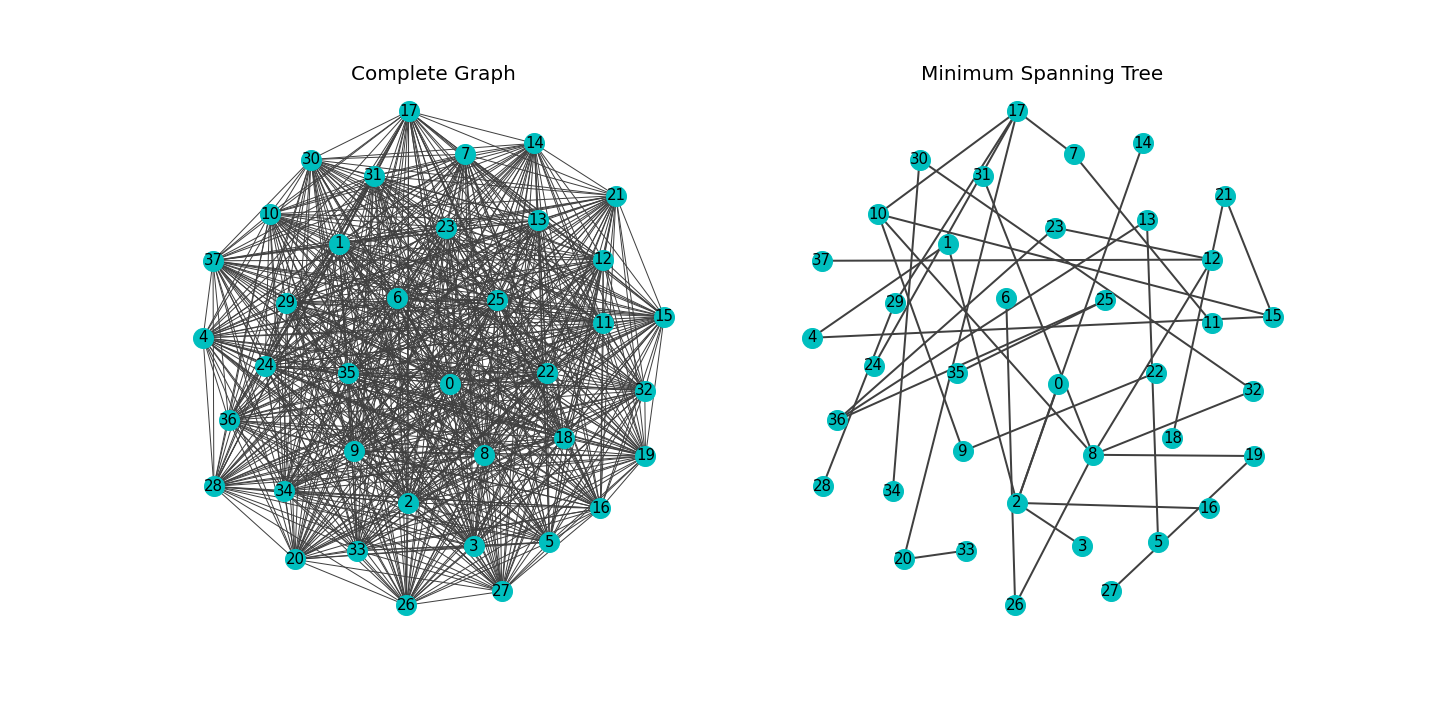
\includegraphics[scale=0.32]{graph_and_mst_no_fuel}
\caption{Product Category Graph and MST}
\label{fig:graph_mst}
\end{figure}
With the correlation matrix transformed using Equation \ref{eq:distance_function}, a graph $G = (V,E)$ was generated such that the vertices $V$ represent the product categories, and the edges $E$ the associations between them. Employing Kruskal's algorithm, a minimum spanning tree was then extracted from this graph. Both the complete graph and the MST are illustrated in Figure \ref{fig:graph_mst}. The value of each node is an integer, which corresponds with the index of the product category in the binary purchase vector dataset. The length of each edge is directly proportionate to its value, such that the greater the value, the greater the length of the edge.



\section{Markov Clustering}
The MST was then clustered using the Markov Clustering algorithm. To identify the most modular clustering configuration (modularity being the minimality of connectedness between dense clusters), an array of inflation scores between $1.5$ and $2.5$ (inclusive) were tested at increments of $0.1$, leading us to determine that an inflation score of $1.6$ resulted in the most optimal modularity. The Markov Clustering was performed using this inflation score, and the clustering results are illustrated in Figure \ref{fig:clustered} (note that while the disposition of the nodes is different from that illustrated in Figure \ref{fig:graph_mst}, the values of all nodes and edges are the same). 
\begin{figure}[H]
\centering
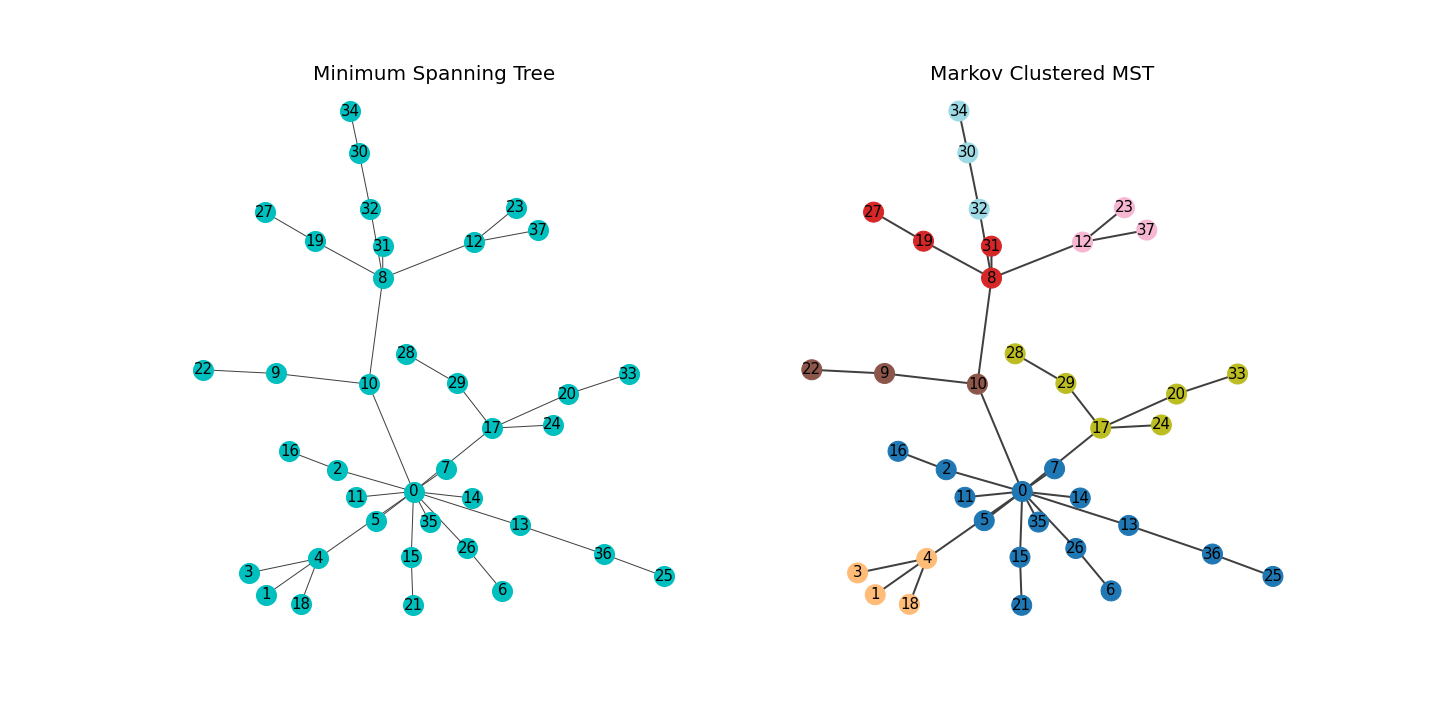
\includegraphics[scale=0.32]{mst_clustered_no_fuel2}
\caption{MST before and after Markov Clustering}
\label{fig:clustered}
\end{figure}
The Markov Clustering algorithm segmented the nodes into 8 distinct clusters.
Figure \ref{fig:cluster_named} illustrates the names of the product categories in each cluster, color-coded in accordance with the graphs in Figure \ref{fig:clustered}.

\begin{figure}[H]
\centering
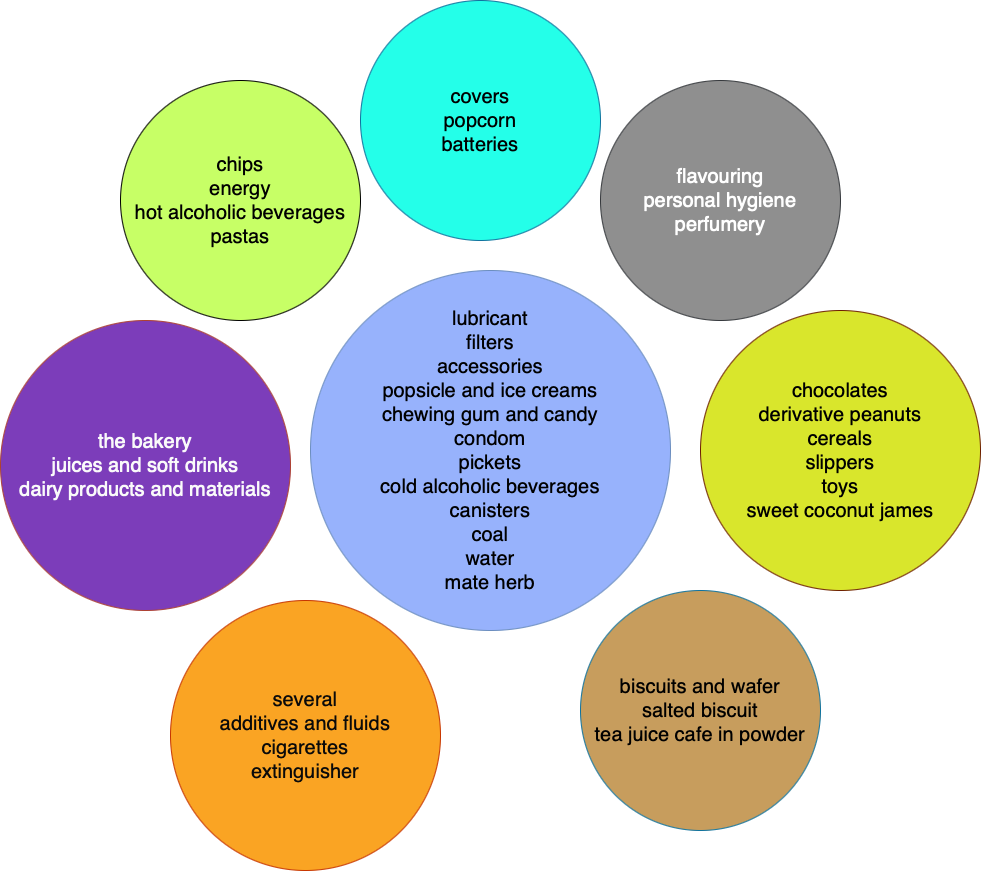
\includegraphics[scale=0.3]{cluster_named}
\caption{Product categories by cluster}
\label{fig:cluster_named}
\end{figure}

\section{Rule Generation}

\subsection{Itemset Generation}
For every cluster identified, all possible itemsets are generated for the $n$ product categories in a given cluster such that the length of the itemsets range from $1$ to $n-1$. Listing \ref{lst:itemset_generation} is the excerpt of code that generates all possible itemsets for a cluster.

\begin{lstlisting}[language=Python, caption=Cluster Itemset Generation, label=lst:itemset_generation]
# Source: arm_cython.pyx
from itertools import combinations
...
cpdef __generate_itemsets_by_cluster():
    global itemsets_by_cluster
    cdef set items
    for index, cluster in enumerate(clusters):
        items = set()
        for set_size in range(1, len(cluster)):
            items.update(combinations(cluster, set_size))
        itemsets_by_cluster[index] = items
\end{lstlisting}
Once the minimum spanning tree has been successfully clustered, association rules can be generated from the clusters in two distinct ways.
\subsection{Bi-Cluster Rule Generation}
Bi-cluster rules are those where the antecedent and consequent originate from distinct and separate clusters. All possible bi-cluster permutations $^nP_2$ are calculated for $n$ clusters. Possible association rules are then generated for these combinations of clusters.


\begin{lstlisting}[language=Python, caption=Cluster Itemset Generation, label=lst:bi_cluster]
# Source: arm_cython.pyx
cpdef list generate_bicluster_rules(min_support=0.005, min_confidence=0.6):
    cdef list rules = []
    cdef list cluster_combinations = list(combinations(list(range(len(clusters))), 2))

    for comb in cluster_combinations:
        a_items = itemsets_by_cluster[comb[0]]
        b_items = itemsets_by_cluster[comb[1]]
        current_rules = list(product(a_items, b_items))
        rules.extend(current_rules)
    
    rules = __add_reverse(rules)
    return __filter_rules(rules, min_support=min_support, min_confidence=min_confidence)
\end{lstlisting}
Listing \ref{lst:bi_cluster} is the excerpt of code used to generate all the bi-cluster rules. On line $4$, we have used the \texttt{combinations} function instead of \texttt{permutations}. 

If we were to use permutations, we would have to generate each itemset $i$ such that: \[\{i_1 \in A\} \rightarrow \{i_2 \in B\}\] for clusters $A$ and $B$, and then later: \[\{i_1 \in B\} \rightarrow \{i_2 \in B\}\] which would essentially be the same combinations in a different configuration. Instead, by using \texttt{combinations} on line $4$ of Listing \ref{lst:bi_cluster}, we only compute the former, and then re-add the rule to the ruleset with the antecedent and consequent swapped (line $12$). This method essentially reduces our computational time by half.

\subsection{Intra-Cluster Rule Generation}
Intra-cluster rules are those where the both antecedent and consequent originate from the same cluster. Similar to the bi-cluster rules, the intra-cluster rules used the itemsets generated via the \texttt{\_\_generate\_itemsets\_by\_cluster()} function in Listing \ref{lst:itemset_generation}, however with the constraint:
\[\{i_1\} \rightarrow \{i_2\}; i \in A\] for every itemset $i$ in cluster $A$.

\subsection{Rule Pruning}
As described in Section \ref{mba_define}, the \textit{anti-monotone property of support} implies that the support for a subset of a given set should be equal to or greater than the support of the set: \[\text{support}(\{x,y\}) \geq \text{support}(\{x,y,z\})\]
To take advantage of this, we first sort our rules in ascending order by the number of elements in the antecedent. When iterating through the potential rules, if either the antecedent or consequent is found to have a support score below the pre-defined minimum tolerance, the itemsets are added to a set \texttt{below\_threshold}. Any future rules iterated are then cross-checked against \texttt{below\_threshold}, 
and if it is found that any set in \texttt{below\_threshold} is a subsset of the rule, the rule is discarded as we know that its support is below our minimum tolerance. This allows us to avoid computing the support for several rules - the time complexity of which $O(n)$ at worst, thereby significantly reducing computation time.
